\chapter{Mengenal Python dan Anaconda}
Tujuan pembelajaran pada pertemuan pertama antara lain:
\begin{enumerate}
\item
Mengerti sejarah python, perkembangan dan penggunaan python di perusahaan
\item
Memahami tahapan instalasi python dan anaconda
\item
Memahami cara penggunaan spyder
\end{enumerate}
Tugas dengan cara dikumpulkan dengan pull request ke github dengan menggunakan format latex pada repo yang dibuat oleh asisten IRC.

\section{Teori}
Praktek teori penunjang yang dikerjakan :
\begin{enumerate}
\item
Buat Resume Sejarah Python, perbedaan python 2 dan 3, dengan bahasa yang mudah dipahami dan dimengerti. Buatan sendiri bebas plagiat(10)
\item
Buat Resume Implementasi dan penggunaan Python di perusahaan dunia, bahasa yang mudah dipahami(10)
\end{enumerate}

\section{Instalasi}
Melakukan instalasi python dan anaconda versi 3 serta uji coba spyder. Dengan menggunakan bahasa yang mudah dimengerti dan bebas plagiat. 
Dan wajib skrinsut dari komputer sendiri.
\begin{enumerate}
\item
Instalasi python 3 (5)
\item
instalasi pip(5)
\item
cara setting environment (5)
\item
mencoba entrepreter/cli melakui terminal atau cmd windows(5)
\item 
Menjalankan dan mengupdate anaconda dan spyder(5)
\item
Cara menjalankan Script hello word di spyder(5)
\item
Cara menjalankan Script otomatis login aplikasi akademik dengan library selenium dan inputan user(5)
\item
Cara pemakaian variable explorer di spyder(5)
\end{enumerate}


\section{Identasi}
Membuat file main.py dan mengisinya dengan script contoh python penggunaan selenium(minimal 20 baris) yang melibatkan inputan user, kemudian mencoba untuk mengatasi error identasi.
\begin{enumerate}
	\item
Penjelasan Identasi (10)
	\item
jenis jenis error identasi yang didapat(10)
\item
cara membaca error(10)
\item 
cara menangani errornya(10)
\end{enumerate}

\section{Presentasi Tugas}
Pada pertemuan ini, diadakan tiga penilaiain yaitu penilaian untuk tugas mingguan dengan nilai maksimal 100. Kemudian dalam satu minggu kedepan maksimal sebelum waktu mata kuliah. Ada presentasi kematerian dengan nilai presentasi yang terpisah masing-masing 100. Dan nilai terpisah untuk tutorial dari jawaban tugas di YouTube.Jadi ada tiga komponen penilaiain pada pertemuan ini yaitu :
\begin{enumerate}
	\item tugas minggu hari ini dan besok (maks 100). pada chapter ini
	\item presentasi csv (maks 100). Mempraktekkan kode python dan menjelaskan cara kerjanya.
	\item pembuatan video tutorial youtube tentang tutorial dari jawaban tugas.(nilai maks 100)
\end{enumerate}
Waktu presentasi pada jam kerja di IRC. Kriteria penilaian presentasi sangat sederhana, presenter akan ditanyai 20(10 pertanyaan program, 10 pertanyaan teori) pertanyaan tentang pemahamannya menggunakan python dan program agan dibuat error hingga presenter bisa menyelesaikan errornya. jika presenter tidak bisa menjawab satu pertanyaan asisten maka nilai nol. Jika semua pertanyaan bisa dijawab maka nilai 100. Presentasi bisa diulang apabila gagal, sampai bisa mendapatkan nilai 100 dalam waktu satu minggu kedepan.

\section{Jawaban Teori}
\begin{enumerate}
    \item Python dikembangkan oleh Guido van Rossum pada tahun 1990 di Stichting Mathematisch Centrum (CWI), Amsterdam sebagai kelanjutan dari bahasa pemrograman ABC. Versi terakhir yang dikeluarkan CWI adalah 1.2.
    \par
    Tahun 1995, Guido pindah ke CNRI di Virginia Amerika sambil terus melanjutkan pengembangan Python. Versi terakhir yang dikeluarkan adalah 1.6. Tahun 2000, Guido dan para pengembang inti Python pindah ke BeOpen.com yang merupakan sebuah perusahaan komersial dan membentuk BeOpen PythonLabs. Python 2.0 dikeluarkan oleh BeOpen. Setelah mengeluarkan Python 2.0, Guido dan beberapa anggota tim PythonLabs pindah ke DigitalCreations.
    \par
    Saat ini pengembangan Python terus dilakukan oleh sekumpulan pemrogram yang dikoordinir Guido dan Python Software Foundation. Python Software Foundation adalah sebuah organisasi non-profit yang dibentuk sebagai pemegang hak cipta intelektual Python sejak versi 2.1 dan dengan demikian mencegah Python dimiliki oleh perusahaan komersial. Saat ini distribusi Python sudah mencapai versi 2.7.14 dan versi 3.6.3
    \par
    Nama Python dipilih oleh Guido sebagai nama bahasa ciptaannya karena kecintaan Guido pada acara televisi Monty Python's Flying Circus. Oleh karena itu seringkali ungkapan-ungkapan khas dari acara tersebut seringkali muncul dalam korespondensi antar pengguna Python.
    \item Beberapa platform populer seperti Spotify dan Netflix adalah contoh platform yang telah memanfaatkan Python dalam analisis data. Penerapan dalam kedua platform ini, utamanya terlihat pada bagaimana Spotify merekomendasikan lagu dan Netflix merekomendasikan film kepada para pelanggannya. Berikut ini adalah beberapa poin penting tentang penggunaan Python dalam analisis data Spotify:
    \par
    \begin{itemize}
        \item Tim Spotify memanfaatkan analitis. Mereka memanfaatkan Luigi, modul dari Python, yang disinkronisasi dengan Hadoop, sebuah framework berbasis Java yang memungkinkan pemrosesan data dengan ukuran sangat besar.
        \item Luigi memungkinkan kamu untuk membangun pipeline yang kompleks dengan cepat. Ini menangani bundling library yang dibutuhkan, serta mengembalikan error log ke komputer lokalmu.
        \item Spotify juga mengaplikasikan Luigi bersama dengan berbagai algoritme machine learning untuk menghidupkan fitur Radio dan Discover, serta rekomendasi untuk orang yang mungkin ingin kamu ikuti.
    \end{itemize}
\end{enumerate}

\section{Jawaban Instalasi}
\begin{enumerate}
    \item Berikut adalah langkah-langkah dalam meninstall Python
    \par
    \begin{itemize}
    \item Sebelum menginstall python anda harus mendownload terlebih dahulu filenya yang ada di google. Disini saya mendownload phyton versi 3.4.2 lalu klik file tersebut seperti pada gambar\ref{python1}
    \begin{figure}[!htbp]
    \centering 
    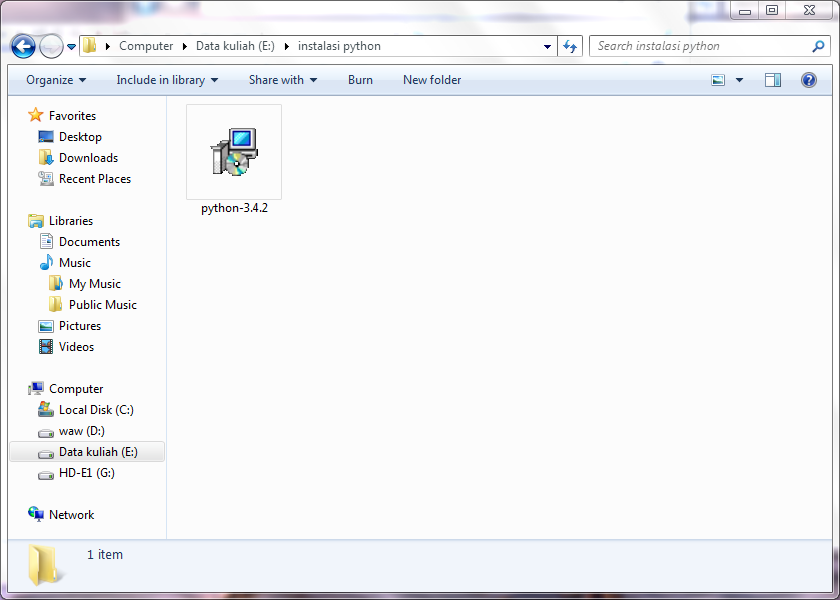
\includegraphics[scale=0.4]{figures/python1.PNG} 
    \caption{\textit{Phyton 3.4.2}}
    \label{python1}
\end{figure}
    \item Pada tahapan ini kita akan diminta untuk memilih siapa saja yang boleh memakai python. Pilih saja ‘Install for all users’ agar bisa dipakai untuk semua user di komputernya seperti pada gambar \ref{python2}
    \begin{figure}[!htbp]
    \centering 
    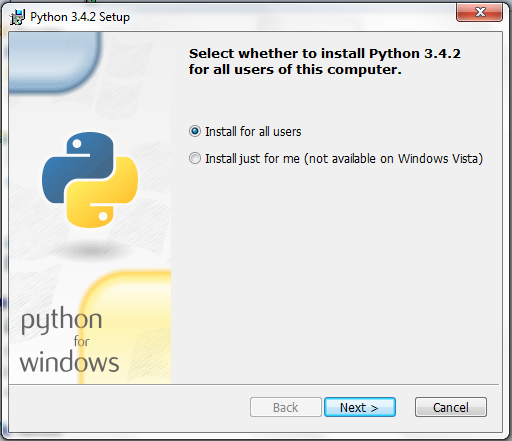
\includegraphics[scale=0.5]{figures/python2.PNG} 
    \caption{\textit{Phyton 3.4.2}}
    \label{python2}
    \end{figure}
    \item Disini kita menentukan lokasi penginstallan python tersebut, biarkan saja di disk C, kemudian klik next seperti pada gambar \ref{python3}
    \begin{figure}[!htbp]
    \centering 
    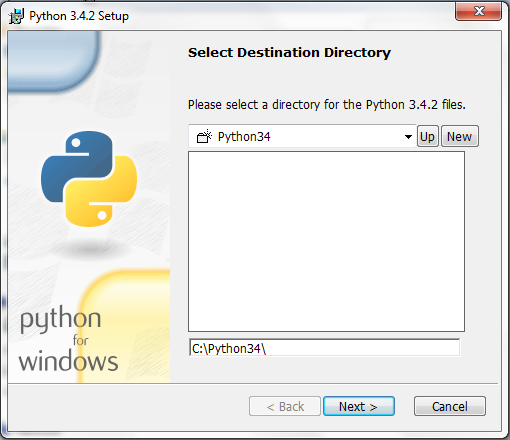
\includegraphics[scale=0.5]{figures/python3.PNG} 
    \caption{\textit{Phyton 3.4.2}}
    \label{python3}
    \end{figure}
    \item Pada tahap ini kita akan menentukan fitur-fitur yang akan diinstall. Jangan lupa untuk mengaktifkan \textit{Add python.exe to path} agar perintah-perintah python dapat dikenali oleh CMD(Command Prompt) seperti pada gambar berikut \ref{python4}
    \begin{figure}[!htbp]
    \centering 
    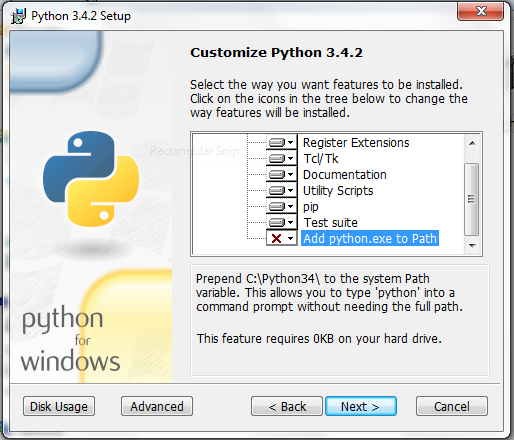
\includegraphics[scale=0.5]{figures/python4.PNG} 
    \caption{\textit{Phyton 3.4.2}}
    \label{python4}
    \end{figure}
    \par Setelah diaktifkan akan menjadi seperti gambar berikut \ref{python5}
    \begin{figure}[!htbp]
    \centering 
    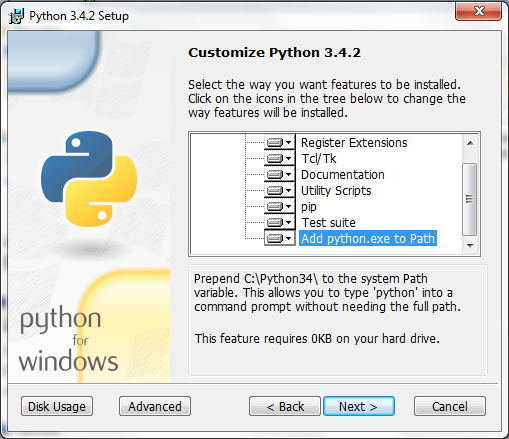
\includegraphics[scale=0.5]{figures/python5.PNG} 
    \caption{\textit{Phyton 3.4.2}}
    \label{python5}
    \end{figure}
    \item Setelah itu klik tombol \textit{Finish} untuk menyelesaikan proses instalasi seperti pada gambar\ref{python6}
    \begin{figure}[!htbp]
    \centering 
    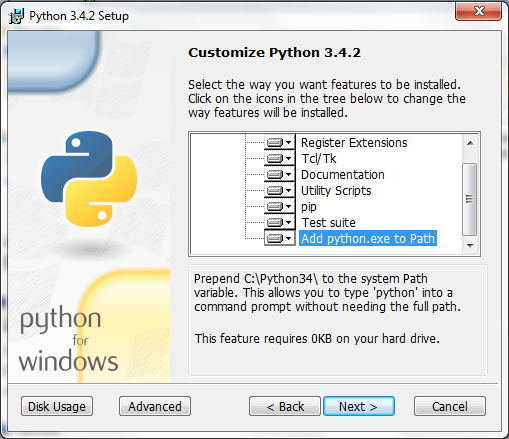
\includegraphics[scale=0.5]{figures/python6.PNG} 
    \caption{\textit{Phyton 3.4.2}}
    \label{python6}
    \end{figure}
\end{itemize}
    
    \item Berikut adalah langkah-langkah dalam menginstall Pip
    \begin{itemize}
        \item Download file pip di situs resminya pip.pypa.io lalu klik kanan dan pilih save link as seperti pada gambar berikut \ref{pip1}
    \begin{figure}[!htbp]
    \centering 
    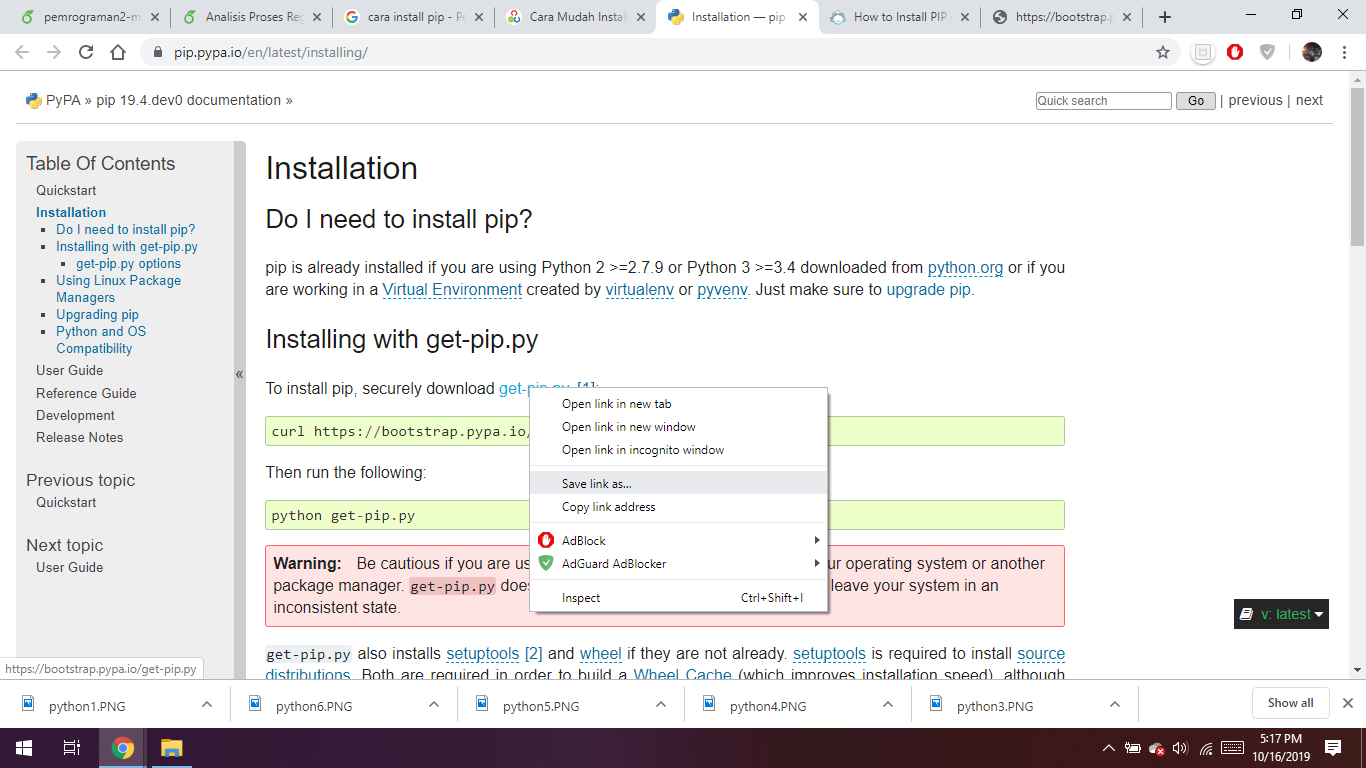
\includegraphics[scale=0.25]{figures/pip1.png} 
    \caption{\textit{get-pip.py}}
    \label{pip1}
    \end{figure}
    \item Selanjutnya klik kanan pada file tersebut dan pilih opsi open with seperti pada gambar \ref{pip2}
    \begin{figure}[!htbp]
    \centering 
    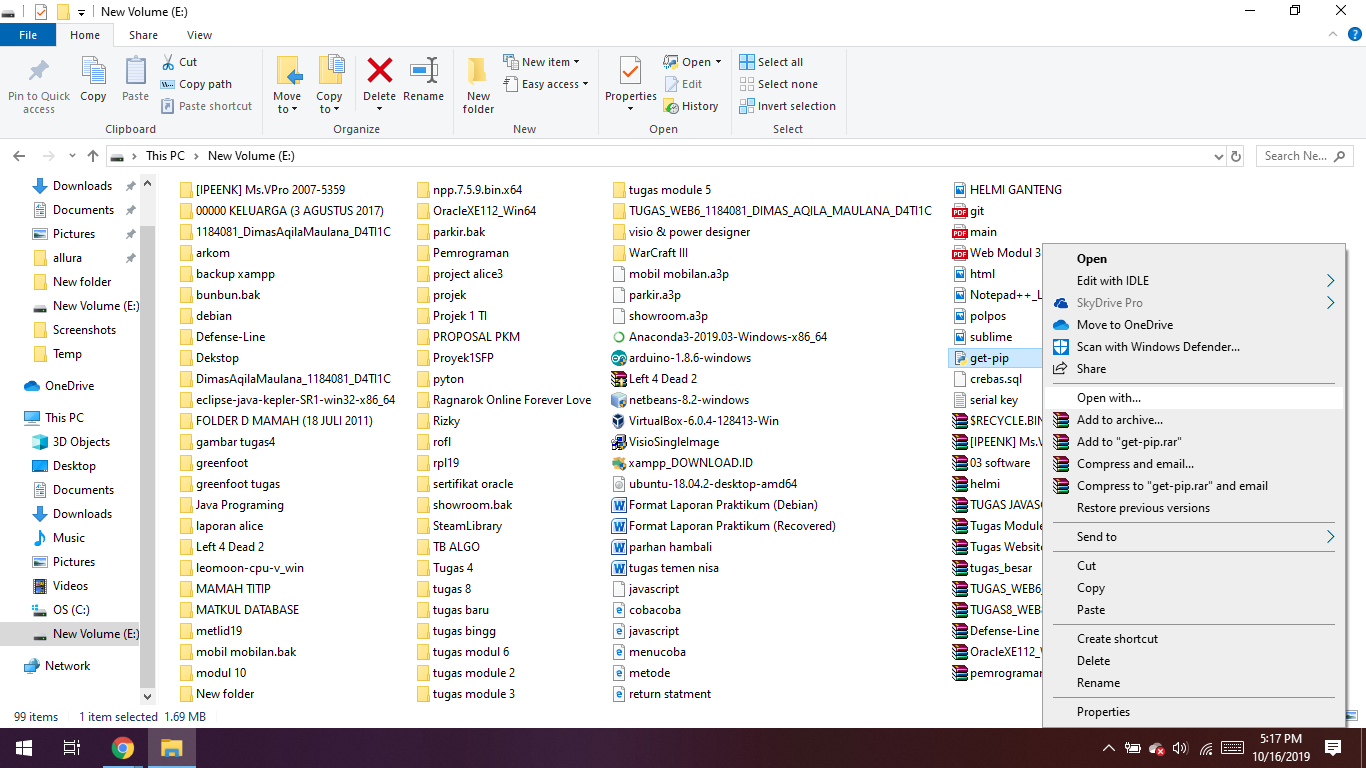
\includegraphics[scale=0.25]{figures/pip2.png} 
    \caption{\textit{get-pip.py}}
    \label{pip2}
    \end{figure}
    \item Lalu buka file tersebut menggunakan Python yang sudah diinstal sebelumnya seperti pada gambar \ref{pip3}
        \begin{figure}[!htbp]
    \centering 
    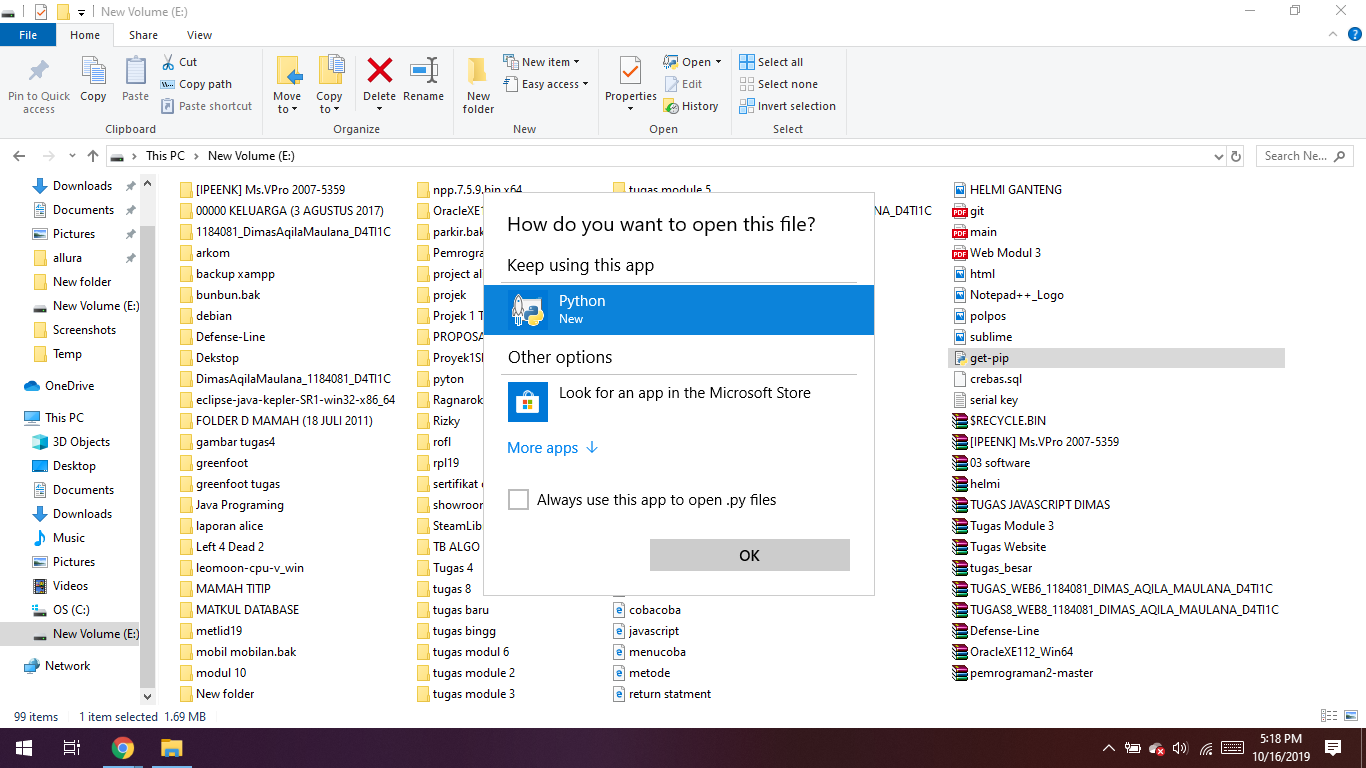
\includegraphics[scale=0.28]{figures/pip3.png} 
    \caption{\textit{get-pip.py}}
    \label{pip3}
    \end{figure}
    \item Setelah itu akan keluar CMD, kita tunggu beberapa saat agar proses instalasi berjalan dengan lancar seperti pada gambar \ref{pip4}
    \begin{figure}[!htbp]
    \centering 
    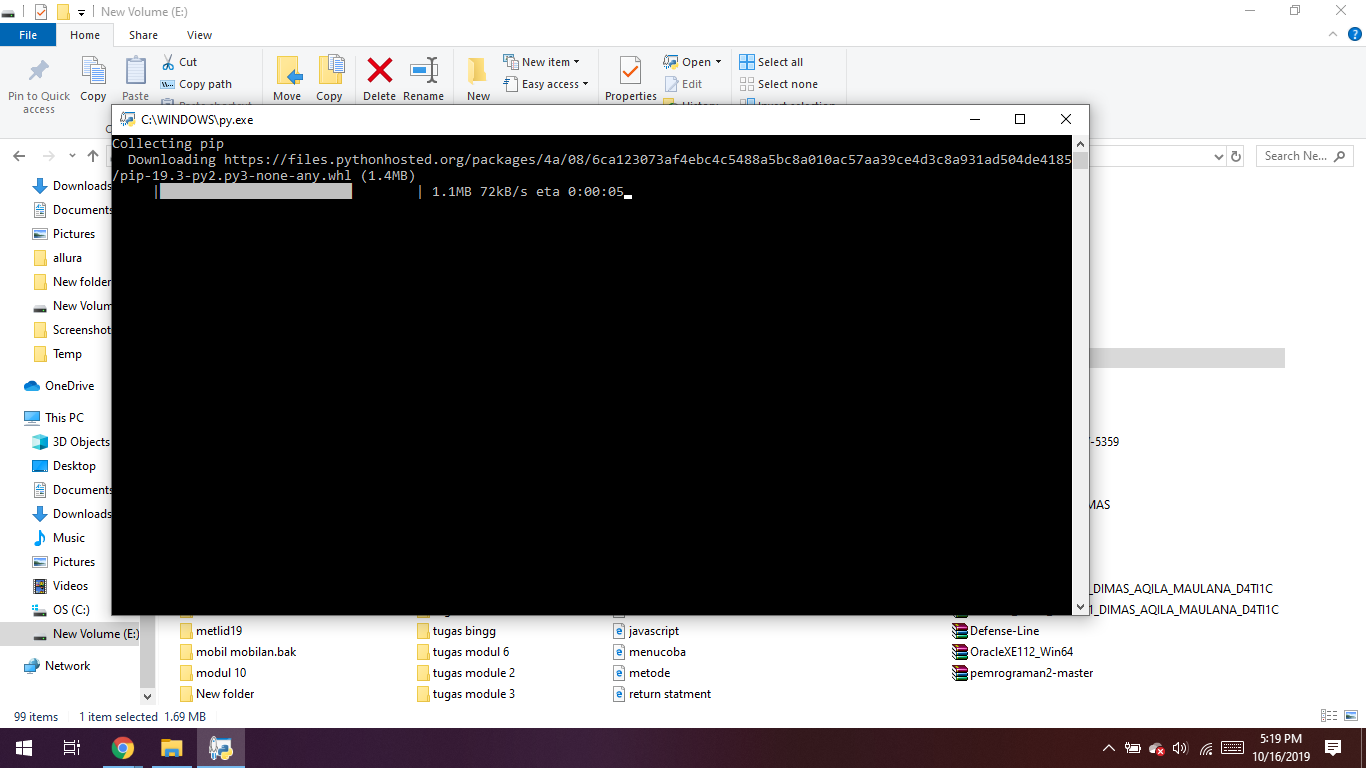
\includegraphics[scale=0.25]{figures/pip4.png} 
    \caption{\textit{get-pip.py}}
    \label{pip4}
    \end{figure}
    \item Saat CMDnya hilang, maka proses instalasi sudah selesai.
    \end{itemize}
    
    \item Cara setting environment
    \begin{itemize}
        \item Buka control panel - system and security - Advance system setting seperti pada gambar \ref{env1}
    \begin{figure}[!htbp]
    \centering 
    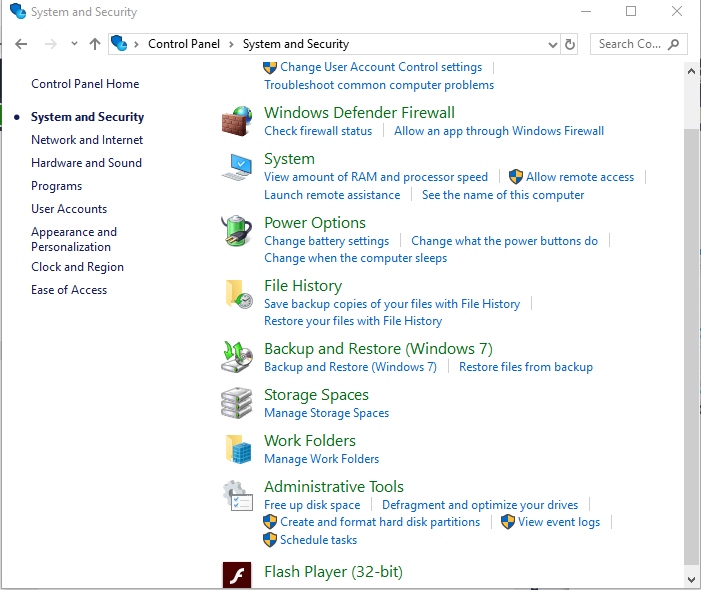
\includegraphics[scale=0.6]{figures/env1.PNG} 
    \caption{Setting Environment}
    \label{env1}
    \end{figure}
    \item Klik Environment Variables pada gambar \ref{env2}
    \begin{figure}[!htbp]
    \centering 
    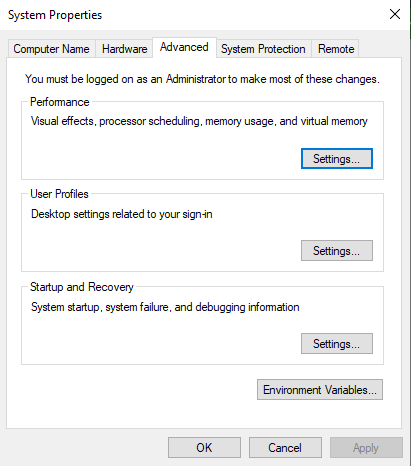
\includegraphics[scale=0.7]{figures/env2.PNG} 
    \caption{Setting Environment}
    \label{env2}
    \end{figure}
    \item Pada bagian Variable scroll sampai bertemu dengan tulisan path dan klik lalu akan ada system edit seperti pada gambar \ref{env3}
        \begin{figure}[!htbp]
    \centering 
    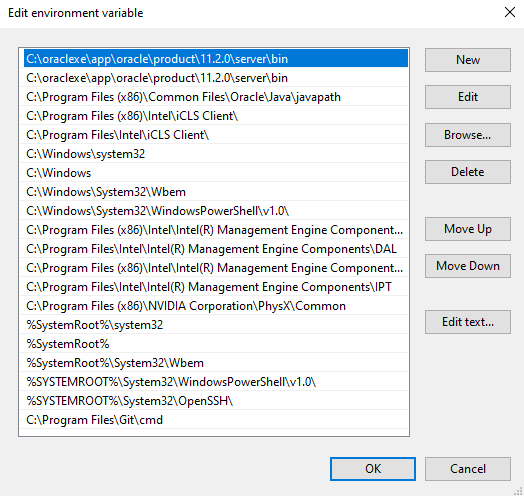
\includegraphics[scale=0.6]{figures/env3.PNG} 
    \caption{Setting Environment}
    \label{env3}
    \end{figure}
    \item Di belakang directory tambahkan huruf ;C:37 tergantung versi python kalian lalu klik ok semuanya seperti gambar \ref{env4}
        \begin{figure}[!htbp]
    \centering 
    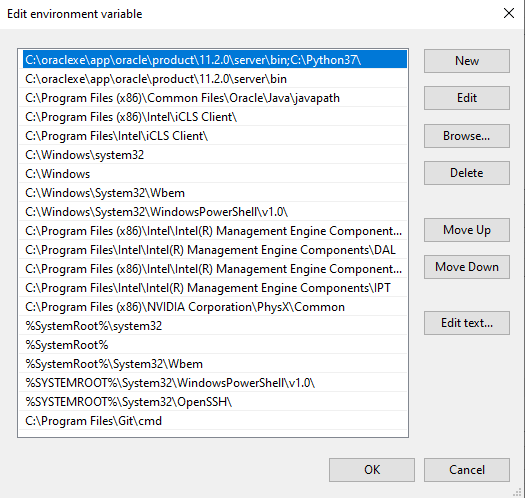
\includegraphics[scale=0.7]{figures/env4.PNG} 
    \caption{Setting Environment}
    \label{env4}
    \end{figure}
    \item Buka cmd lalu ketikkan pip install request dan tunggu hingga proses instalasi selesai seperti pada gambar \ref{env5}
        \begin{figure}[!htbp]
    \centering 
    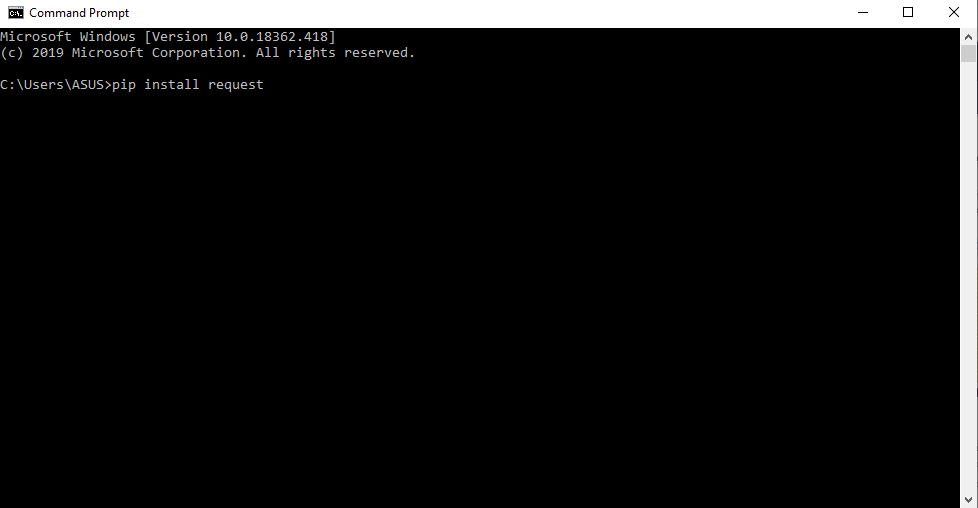
\includegraphics[scale=0.55]{figures/env5.PNG} 
    \caption{Setting Environment}
    \label{env5}
    \end{figure}
    \end{itemize}
    \item Mencoba enterpreter/cli melalui terminal atau cmd windows
    \begin{itemize}
        \item Buka cmd - lalu ketik python - tunggu - ketikan angka 5*5 seperti pada gambar \ref{cli2}
    \begin{figure}[!htbp]
    \centering 
    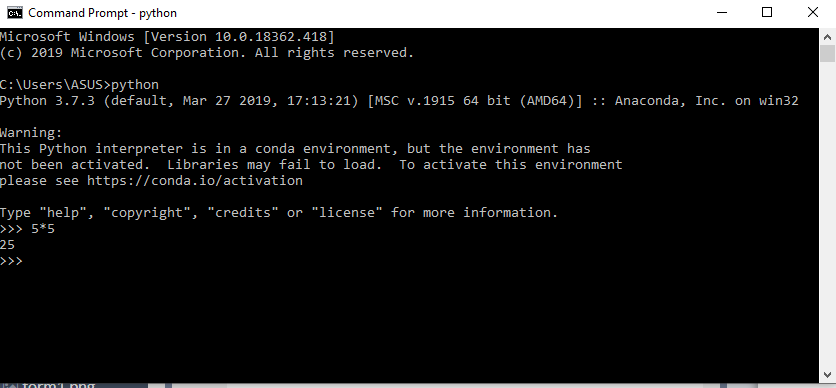
\includegraphics[scale=0.65]{figures/cli2.PNG} 
    \caption{Enterpreter/Cli}
    \label{cli2}
    \end{figure}
    \end{itemize}
    \item Menjalankan dan mengupdate anaconda dan spyder
    \begin{itemize}
        \item Cari aplikasi anaconda navigator pada windows - tunggu beberapa saat - anaconda berhasil di launch seperti pada gambar \ref{anaconda1}
    \begin{figure}[!htbp]
    \centering 
    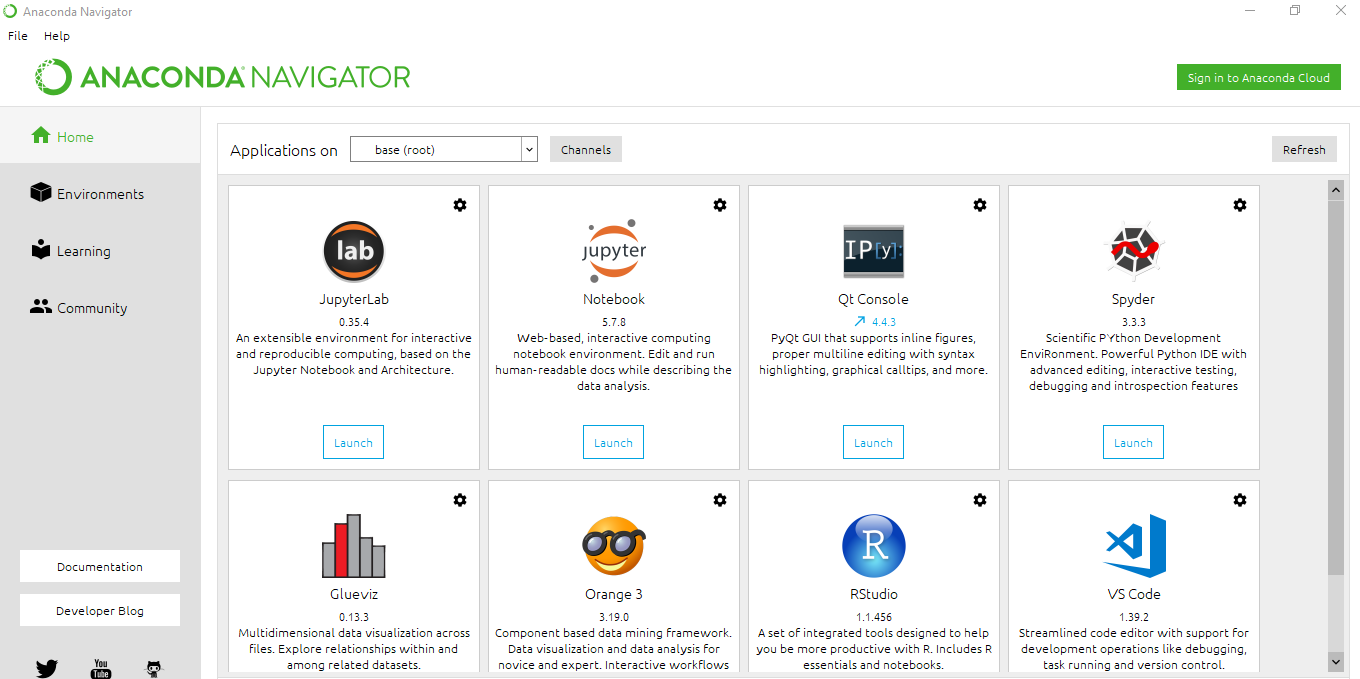
\includegraphics[scale=0.4]{figures/anaconda1.PNG} 
    \caption{Launch Anaconda}
    \label{anaconda1}
    \end{figure}
    \item Setelah launch Anaconda, klik Launch spyder tunggu beberapa saat seperti pada gambar \ref{spy1}
    \begin{figure}[!htbp]
    \centering 
    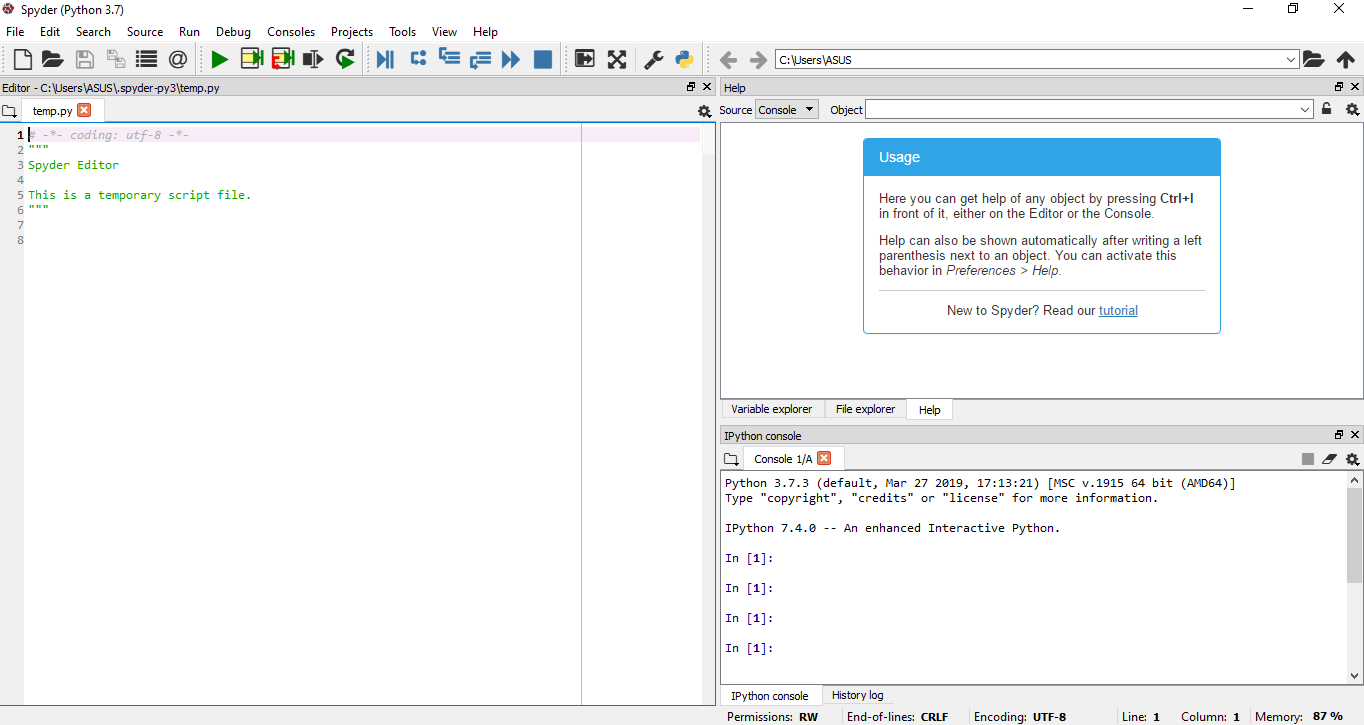
\includegraphics[scale=0.4]{figures/spy1.PNG} 
    \caption{Launch Spyder}
    \label{spy1}
    \end{figure}
    \end{itemize}
    \item Cara menjalankan script hello world di spyder
    \begin{itemize}
        \item Ketikkan print('Hello World') pada kolom 8 lalu klik tombol run seperti pada gambar \ref{spy3}
            \begin{figure}[!htbp]
    \centering 
    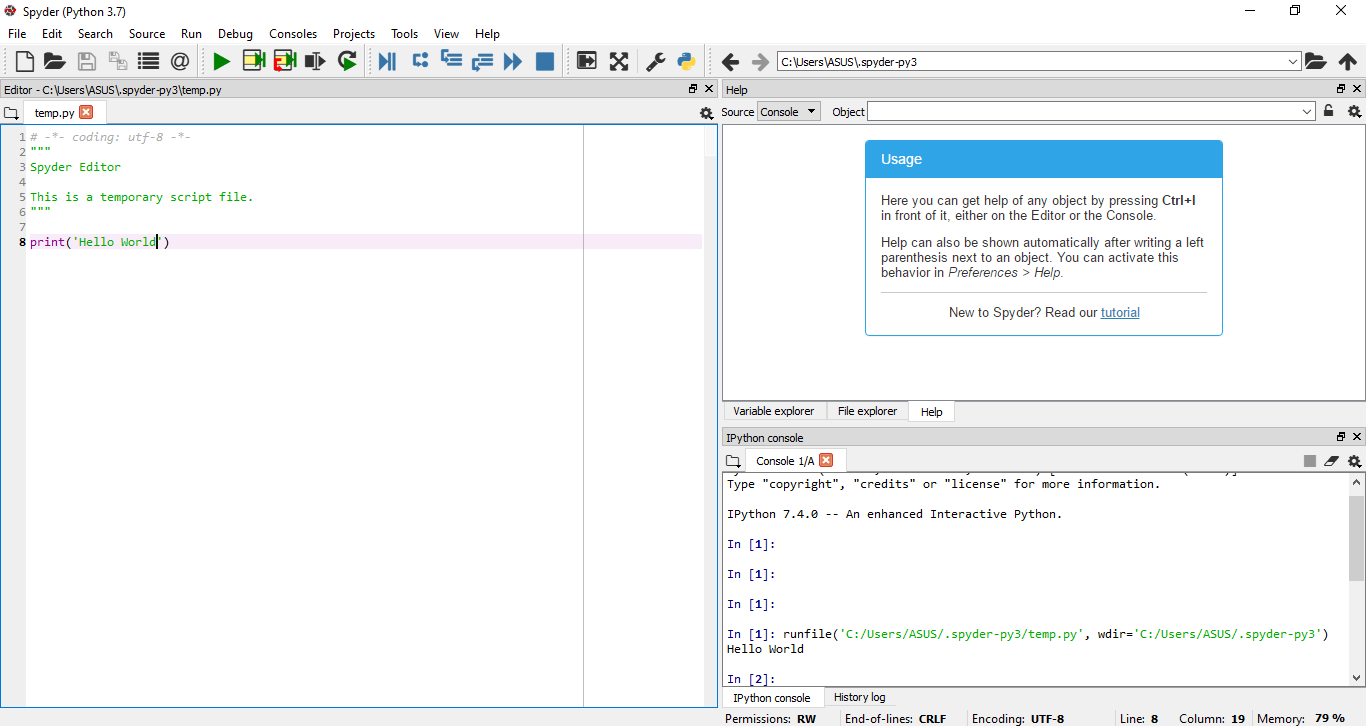
\includegraphics[scale=0.4]{figures/spy3.PNG} 
    \caption{Script Spyder}
    \label{spy3}
    \end{figure}
    \end{itemize}
    \item Cara pemakaian variable explorer di spyder
    \begin{itemize}
        \item Pada aplikasi spyder tuliskan contoh a=7 b=3 c=a*b lalu running script tersebut maka variable explorer akan menerima inputan script tersebut seperti pada gambar \ref{spy4}
    \begin{figure}[!htbp]
    \centering 
    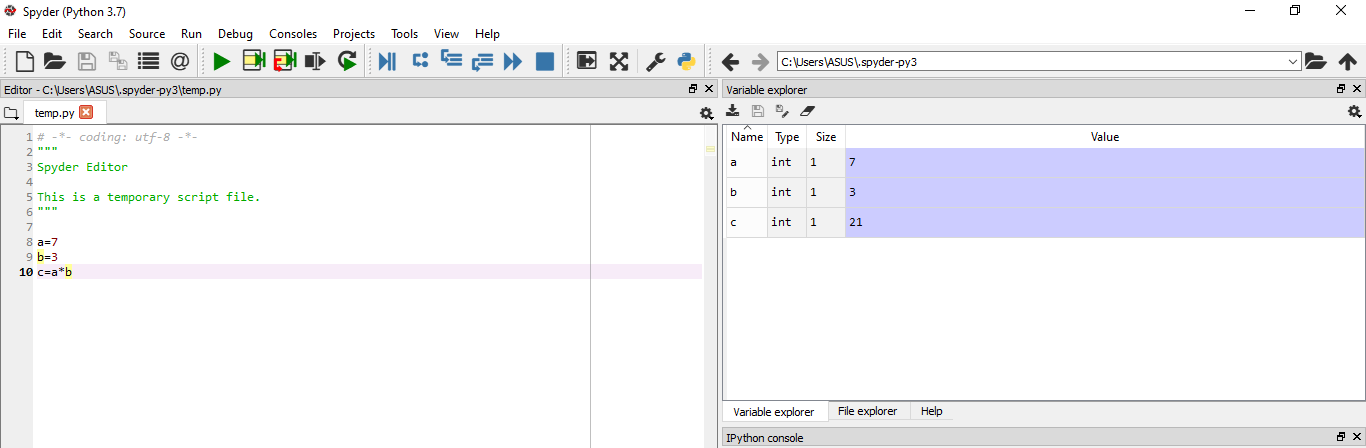
\includegraphics[scale=0.4]{figures/spy4.PNG} 
    \caption{Variable Explorer}
    \label{spy4}
    \end{figure}
    \end{itemize}
\end{enumerate}

\section{Identasi}
\begin{enumerate}
    \item Penjelasan Identasi
    \par
    Indentasi adalah penulisan paragraf yang agak menjorok masuk ke dalam. Indentasi pada umumnya digunakan jika Anda merespon pesan sebelumnya. Untuk membuat indentasi, Anda dapat menambahkan tanda titik dua (:) di awal baris/paragraf. Jika Anda menambah tanda titik dua (:) lagi, maka paragraf akan semakin menjorok.
\end{enumerate}
